\chapter{Single-Lepton Stop Search}
\label{chap:stop}

This chapter will describe a search for supersymmetry with the target signal
being stop-antistop squark pairs decaying to a single-lepton (1$\ell$)
final state. This work was performed using the CMS experiment during
Run II of the LHC, at 13 TeV center-of-mass energy. This analysis
resulted in two publications: the search performed using 2016 data \cite{stop1l},
and a combined single-lepton and all-hadronic search using 2015 data
\cite{combination0l}. Two public research documents (PASes) were
also produced to support conference results \cite{pasichep,pasmoriond},
however these are superceded by the published results. I will focus on
the analysis as described in Reference \cite{stop1l}, particularly my work
developing the compressed T2tt search strategy.

\section{Motivation}
\label{sec:stop:motivation}

As Section \ref{ssec:susy:rationale} has described, supersymmetry
(SUSY) is a very important class of theories in particle physics. It
has the potential to solve the hierarchy problem, and may provide the
answer to the difficult question of what particles make up dark
matter. And the notion of naturalness would seem to imply that our
current or near-future particle colliders have just the right energies
to search for evidence of SUSY.

One particularly interesting feature of SUSY is that if you arrange
the sparticles in order from lightest to heaviest, they will generally line up
in reverse order from the Standard Model particles. So whereas the
electron is the lightest stable SM particle, and the top quark is the
heaviest, by contrast the stop squark is expected to be one of the lightest
sparticles, and the selectron one of the heaviest. We say SUSY has an
\emph{inverted mass hierarchy}. % Cite this!
% See refs 8-12 in 8 TeV stop paper.
This means that the Lightest Supersymmetric Particle ($\lsp$), the
chargino ($\chargino$), and the stop squark ($\tilde{t}$) should be
some of the easiest sparticles to detect.
% The single-lepton channel provides a nice balance between
% cross-section and ease of ID.

\section{Previous Searches}
\label{sec:stop:run1}

A search for stop pairs in the one-lepton final state was previously
performed at CMS during Run I \cite{stop1l8tev}. This search used 19.5
fb$^{-1}$ of 8 TeV collision data. The analyzers performed a traditional
cut-based search, and also a search employing a boosted decision tree
(BDT). This machine-learning technique allows a computer to attempt to
discriminate between signal and background. Ultimately, neither search
strategy detected any evidence of the production of stop squarks. This
result allowed the analyzers to set limits on the possible masses of
stops and LSPs. Specifically, stop squarks were excluded up to masses
of about 650 GeV in the case where the LSP is massless, and LSPs were
excluded up to a maximum of 200-250 GeV for stop masses around 500-600
GeV.

The LHC and the CMS detector received a number of upgrades for Run II,
some of which have greatly benefitted the single-lepton stop
search. Of particular note, the LHC collision energy was raised from 8
to 13 TeV, which increases the likelihood of producing heavy new
particles, and the luminosity was increased considerably, allowing us % Quantify lumi increase
to record more data in the same amount of running time. In addition,
we have learned from the Run I analysis, and attempted to improve our
analysis techniques for Run II. To avoid the obfuscation inherent in
results produced by machine learning, we declined to perform a BDT
search. We also added a new signal model to our search. Finally, we
added dedicated signal regions to address the unique kinematics of
several particular regions of phase space.

% How about any ATLAS stop-1L searches?
% Or searches from CDF or D0?
% It's hard, because there are a LOT of searches that set limits on
% stops in general.

% There's a nice plot in the AN that shows how the predicted cross
% sections increase from 8 -> 13 TeV

\section{Signal Models}
\label{sec:stop:sigmodels}

Because supersymmetry is still a theoretical construct, and the masses
of the sparticles are unknown, there are a number of possible
ways that a stop squark pair could decay to a single lepton final
state. We consider three possible signal models, each with its own
unique signature. In addition, we consider a wide range of possible
masses for our sparticles, and the kinematics that result.

\subsection{Bulk Signals}
\label{ssec:stop:sigbulk}

\subsubsection*{T2tt}

One of the primary models we target is known by the identifer
\textbf{T2tt}. In this model, the stop squarks decay to top quarks and
LSPs ($\tilde{t} \rightarrow t \lsp_1$). The top quarks then decay to
bottoms and W bosons, as normal; one of the Ws decays leptonically,
and the other hadronically. The two free parameters in this model are
the stop mass, $\mstop$, and the LSP mass, $m_{\lsp_0}$; we
scan a wide range of possible values for these two variables. The
kinematics of the decay products are determined entirely by the stop
and LSP masses. A diagram of the T2tt model is pictured at the top of
Figure \ref{fig:stop:feynmandiagrams}.

\subsubsection*{T2bW}

The second primary model we consider is known as \textbf{T2bW}. In this
model, the stop squarks decay to bottom quarks and charginos, skipping
the top quarks entirely. The charginos then decay to W bosons and
neutralinos ($\tilde{t} \rightarrow b \chargino_1, \chargino_1 \rightarrow
W \lsp_1$). One W then decays leptonically, and the other
hadronically. In this case, the free parameters are $\mstop$,
$m_{\lsp_0}$, and also the chargino mass, $\mchargino$. For the
purposes of this analysis, we fix the chargino mass at the average of
the stop and neutralino masses, $\mchargino = (\mstop
+ \mlsp) / 2$. We then scan a broad range of possible values
for $\mstop$ and $\mlsp$. We also created a set of
dedicated signal regions targeting the case where $\mchargino$ and
$\mlsp$ are nearly identical. The T2bW model is diagrammed in
the middle of Figure \ref{fig:stop:feynmandiagrams}.

\subsubsection*{T2tb}

For the Run II search, we have added a new signal model that was not
evaluated in the Run I search. This model is called \textbf{T2tb}. It
is essentially a mixture of the T2tt and T2bW models, in that it
covers the case where one of the stop squarks decays to a top quark
and an LSP, and the other decays to a bottom quark and a chargino. For
this analysis, we fix $\mchargino$ to be $\mlsp + 5$ GeV. We
then scan a range of possible values for $\mstop$ and
$\mlsp$. The T2tb model is pictured at the bottom of Figure
\ref{fig:stop:feynmandiagrams}.

% Insert Feynman diagrams. Either make them, or pull from the documentation.

\subsection{Compressed T2tt}
\label{ssec:stop:sigcompressed}

There is a region of the $\mstop$ and $\mlsp$ phase space
that is of particular interest to us in this analysis. In the T2tt
model, if the difference between the stop and LSP masses is less than
the mass of the top quark, $\mstop - \mlsp \lesssim m_t$, then the top quark
must be produced off-shell (i.e. with a mass that is not its normal
$\sim$173 GeV). This kind of process would be difficult to detect
because the production of off-shell top quarks is suppressed, and
because there is also less energy and momentum available to the top
deca products. We may also consider what happens if we go one step
further, to the region where $\mstop - \mlsp \lesssim m_W$. In this case, not
only the top quark but also its resultant W boson must be produced
off-shell, making it even harder to detect this signal. We call these
cases ``compressed'' T2tt decays, because the phase space available to
the decay products is squeezed down to a smalle range.

The difficulties in detecting compressed T2tt signals are evident in
the results plot of the Run I analysis \cite{stop1l8tev}. The exclusion
curve for the T2tt model has no coverage in the narrow strip where
$\mstop - \mlsp \approx m_t$, or the strip where $\mstop - \mlsp
\approx m_W$. We call these two regions the \emph{top corridor} and
the \emph{W corridor}, respectively. In this analysis we wished to
fill in these two gaps, and achieve exclusion in the corridor
regions. To that end, I developed a specialized set of
signal regions that target the kinematics of compressed decays, with
the aim of increasing our sensitivity to these signals. These
specialized signal regions will be described in Section
\ref{ssec:stop:corridorsrs}, and the compressed T2tt search will be
described separately from the nominal search in cases where
the two strategies differ.

\section{Datasets and Triggers}
\label{sec:stop:datatrig}

\subsection{Data samples}
\label{ssec:stop:datasamples}

There are two main signatures that we use to search for our stop
decays. The first is the presence of a single, isolated lepton. This
signature is fairly obvious, because we chose to search in the single
lepton final state. In addition, all of our signal models have two
LSPs and a neutrino in the final state. The LSPs should go undetected
by the CMS detector, just as neutrinos do, so we also expect our
signals to appear with large amounts of $\met$. % This may no longer be the first place I describe the signature

With these two main signatures in mind, we select our data from the
Single Lepton and $\met$ datasets produced by the CMS
experiment. We also employ the single muon or electron dataset for certain control
regions to be described in Section \ref{ssec:stop:lostlep}, and the
single photon datasets for $\met$ resolution studies to be % Need reference to MET resolution studies
described in Section \ref{}. These datasets were recorded during the
2016 datataking period, encompassing eras 2016B through 2016H, and
represent a total integrated luminosity of 35.9 fb$^{-1}$. Table
\ref{tab:stop:datasets} gives a complete listing of all datasets used
in the analysis.

% Homemade table of datasets goes here. %%%%%%%%%%%%%% Would be nice to add run ranges!
\begin{table}[htbp]
\centering
\caption{List of datasets used in the analysis.}
\label{tab:stop:datasets}
\begin{tabular}{l}
\hline
Dataset \\
\hline
  /SingleMuon/Run2016B-03Feb2017\_ver2-v2/MINIAOD \\
  /SingleMuon/Run2016C-03Feb2017-v1/MINIAOD \\
  /SingleMuon/Run2016D-03Feb2017-v1/MINIAOD \\
  /SingleMuon/Run2016E-03Feb2017-v1/MINIAOD \\
  /SingleMuon/Run2016F-03Feb2017-v1/MINIAOD \\
  /SingleMuon/Run2016G-03Feb2017-v1/MINIAOD \\
  /SingleMuon/Run2016H-03Feb2017\_ver2-v1/MINIAOD \\
  /SingleMuon/Run2016H-03Feb2017\_ver3-v1/MINIAOD \\
\hline
  /SingleElectron/Run2016B-03Feb2017\_ver2-v2/MINIAOD \\
  /SingleElectron/Run2016C-03Feb2017-v1/MINIAOD \\
  /SingleElectron/Run2016D-03Feb2017-v1/MINIAOD \\
  /SingleElectron/Run2016E-03Feb2017-v1/MINIAOD \\
  /SingleElectron/Run2016F-03Feb2017-v1/MINIAOD \\
  /SingleElectron/Run2016G-03Feb2017-v1/MINIAOD \\
  /SingleElectron/Run2016H-03Feb2017\_ver2-v1/MINIAOD \\
  /SingleElectron/Run2016H-03Feb2017\_ver3-v1/MINIAOD \\
\hline
  /MET/Run2016B-03Feb2017\_ver2-v2/MINIAOD \\
  /MET/Run2016C-03Feb2017-v1/MINIAOD \\
  /MET/Run2016D-03Feb2017-v1/MINIAOD \\
  /MET/Run2016E-03Feb2017-v1/MINIAOD \\
  /MET/Run2016F-03Feb2017-v1/MINIAOD \\
  /MET/Run2016G-03Feb2017-v1/MINIAOD \\
  /MET/Run2016H-03Feb2017\_ver2-v1/MINIAOD \\
  /MET/Run2016H-03Feb2017\_ver3-v1/MINIAOD \\
\hline
  /MuonEG/Run2016B-03Feb2017\_ver2-v2/MINIAOD \\
  /MuonEG/Run2016C-03Feb2017-v1/MINIAOD \\
  /MuonEG/Run2016D-03Feb2017-v1/MINIAOD \\
  /MuonEG/Run2016E-03Feb2017-v1/MINIAOD \\
  /MuonEG/Run2016F-03Feb2017-v1/MINIAOD \\
  /MuonEG/Run2016G-03Feb2017-v1/MINIAOD \\
  /MuonEG/Run2016H-03Feb2017\_ver2-v1/MINIAOD \\
  /MuonEG/Run2016H-03Feb2017\_ver3-v1/MINIAOD \\
\hline
  /SinglePhoton/Run2016B-03Feb2017\_ver2-v2/MINIAOD \\
  /SinglePhoton/Run2016C-03Feb2017-v1/MINIAOD \\
  /SinglePhoton/Run2016D-03Feb2017-v1/MINIAOD \\
  /SinglePhoton/Run2016E-03Feb2017-v1/MINIAOD \\
  /SinglePhoton/Run2016F-03Feb2017-v1/MINIAOD \\
  /SinglePhoton/Run2016G-03Feb2017-v1/MINIAOD \\
  /SinglePhoton/Run2016H-03Feb2017\_ver2-v1/MINIAOD \\
  /SinglePhoton/Run2016H-03Feb2017\_ver3-v1/MINIAOD \\
\hline
\end{tabular}
\end{table}

\subsection{Triggers}
\label{ssec:stop:triggers}

For each of the datasets described above, we select events using
appropriate HLT triggers. Of particular note, we select data events
for our signal regions using the union of the single lepton and $\met$
triggers. This strategy allows us to use leptons that are below their
trigger thresholds, and to compensate for any inefficiency in the
turn-on phase of the $\met$ trigger. The triggers we use are
listed in Table \ref{tab:stop:trigs}.

% Table of HLT triggers paths, adapted from AN-14-463, with a few modifications
\begin{table}[htb]
\caption{HLT trigger paths corresponding to each of the primary
  datasets used in the analysis. The trigger version is suppressed.}
\label{tab:stop:trigs}
\centering
\footnotesize
\begin{tabular}{|l|l|}
\hline
Type & HLT path \\
\hline
SingleMuon & HLT\_Iso(Tk)Mu22 OR HLT\_Iso(Tk)Mu24 \\
SingleElectron & HLT\_Ele25\_eta2p1\_WPTight\_Gsf OR HLT\_Ele27\_eta2p1\_WPTight\_Gsf \\
\hline
\multirow{3}{*}{MET} & HLT\_PFMET170\_HBHECleaned OR \\
 & HLT\_PFMET(NoMu)110\_PFMHT110(NoMu)\_IDTight OR \\
 & HLT\_PFMET(NoMu)120\_PFMHT120(NoMu)\_IDTight \\
\hline
\hline
\multirow{2}{*}{MuonEG} & HLT\_Mu8\_TrkIsoVVL\_Ele23\_CaloIdL\_TrackIdL\_IsoVL(\_DZ) OR \\ 
 & HLT\_Mu23\_TrkIsoVVL\_Ele12\_CaloIdL\_TrackIdL\_IsoVL(\_DZ) \\
\hline
\multirow{2}{*}{SinglePhoton} & HLT\_Photon*\_R9Id90\_HE10\_IsoM OR HLT\_Photon165\_HE10 OR \\
 & HLT\_Photon175 OR HLT\_Photon250\_NoHE \\
\hline
\end{tabular}
\end{table}

\subsection{Trigger efficiency measurements}
\label{ssec:stop:trigeff}

% It kinda helps to know what the lost lepton background is before
% this section
We measure the efficiency of our combined single lepton and $\met$
triggers in a sample of events from the JetHT primary dataset,
selected using the \verb+HLT_(PF)HT*+ trigger paths. We use events
triggered on $H_T$ because this trigger is expected to be orthogonal
to the $\met$ and lepton $p_T$ triggers, allowing us to examine the full % Should I actually say how the efficiency is computed?
spectrum of these variables. The trigger
efficiency is parameterized in $\met$ and lepton $p_T$. We select events
with at least one lepton and two jets. Our definitions of leptons,
jets, and $\met$ are presented later, in Section
\ref{sec:stop:selections}.

Figure \ref{fig:stop:trigeff:1lepmet} shows the parameterized trigger
efficiencies, separated by flavor of the leading lepton. Using 35.9 fb$^{-1}$
of data, our overall trigger efficiency is 99.1\% in the region $\met >$
250 GeV and lepton $p_T >$ 20 GeV. Because this efficiency is so close
to 100\%, we do not correct for the small inefficiency. However, we
assign a systematic uncertainty of 2\% for events with $\met$ below 300
GeV, and 4\% for events with $\met$ greater than 300 GeV.

% Plots of trigger efficiency taken from AN-16-463. Unpublished!
\begin{figure}[htb]
\centering
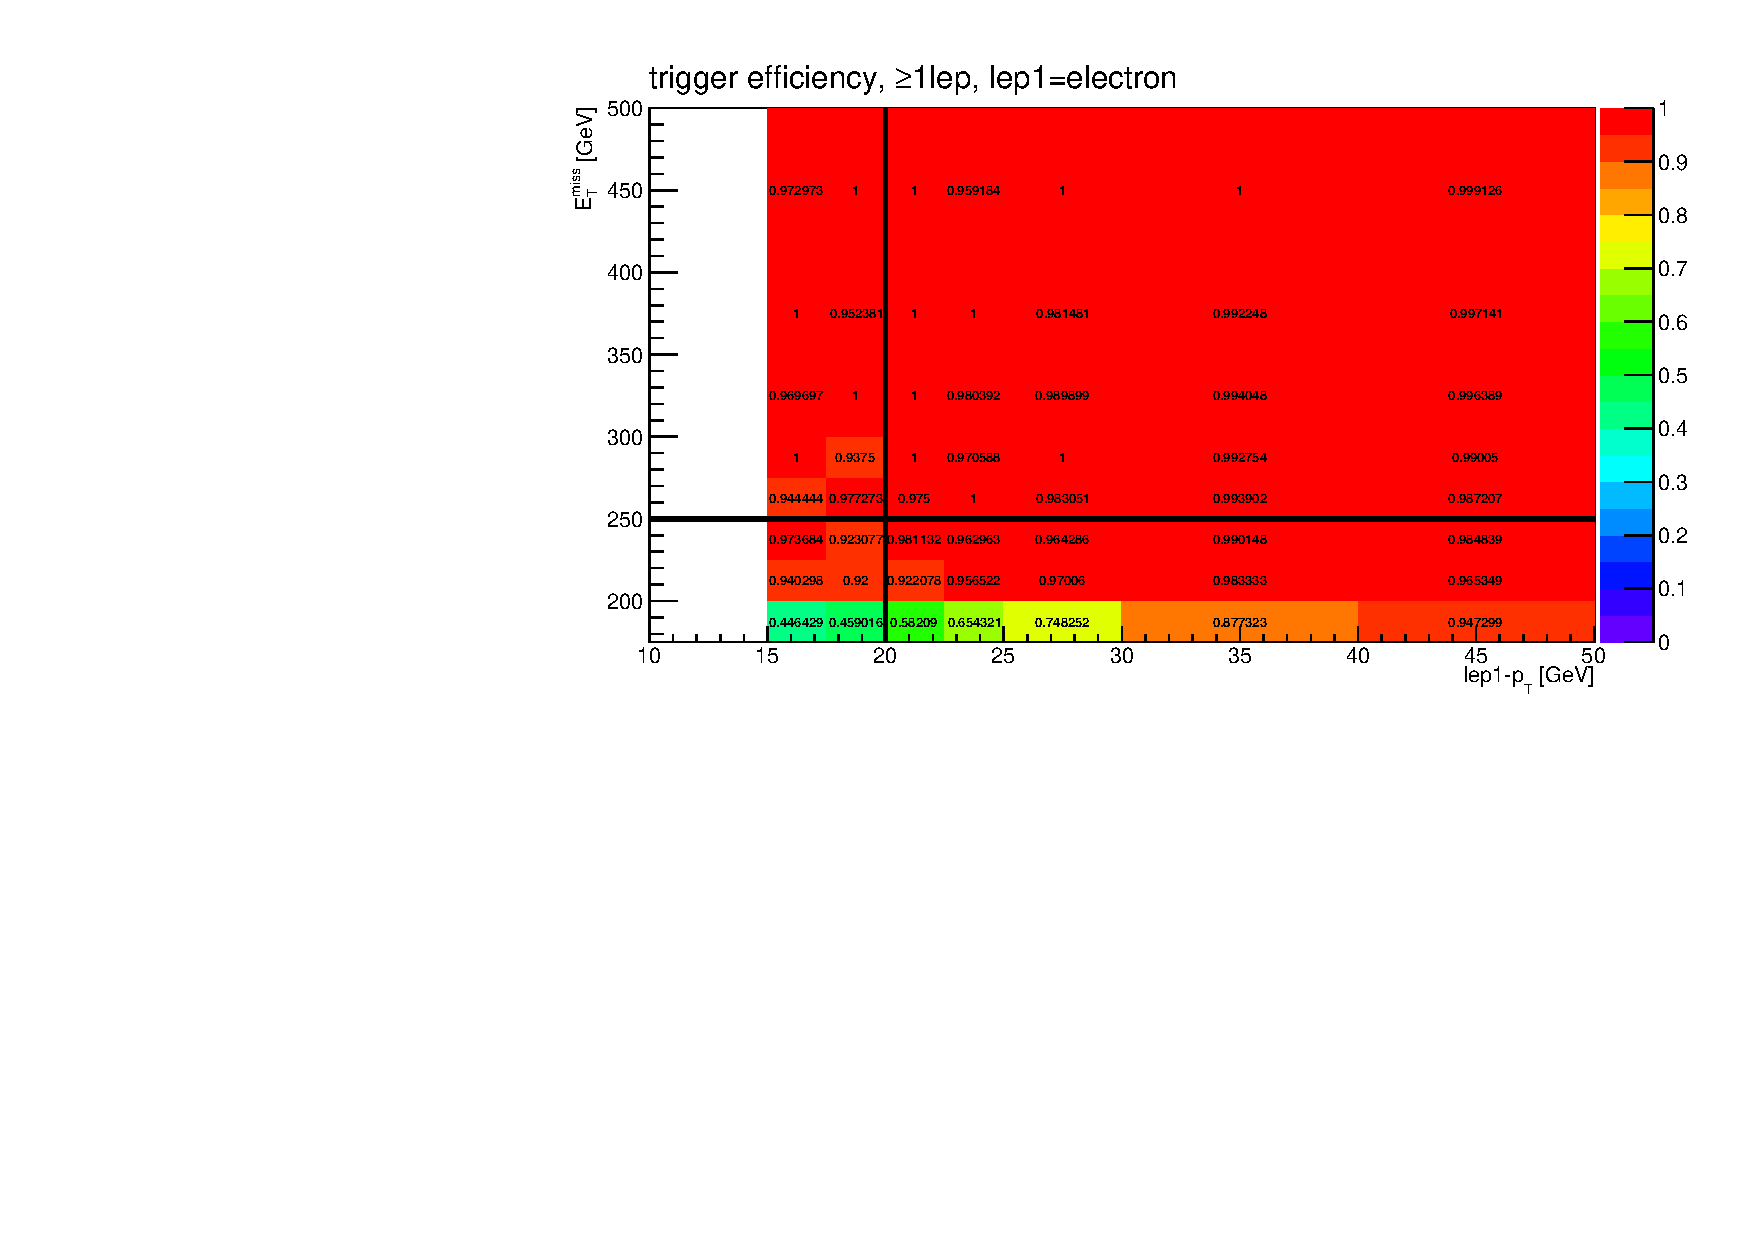
\includegraphics[width=0.45\textwidth]{figures/TriggerEff_el.pdf}
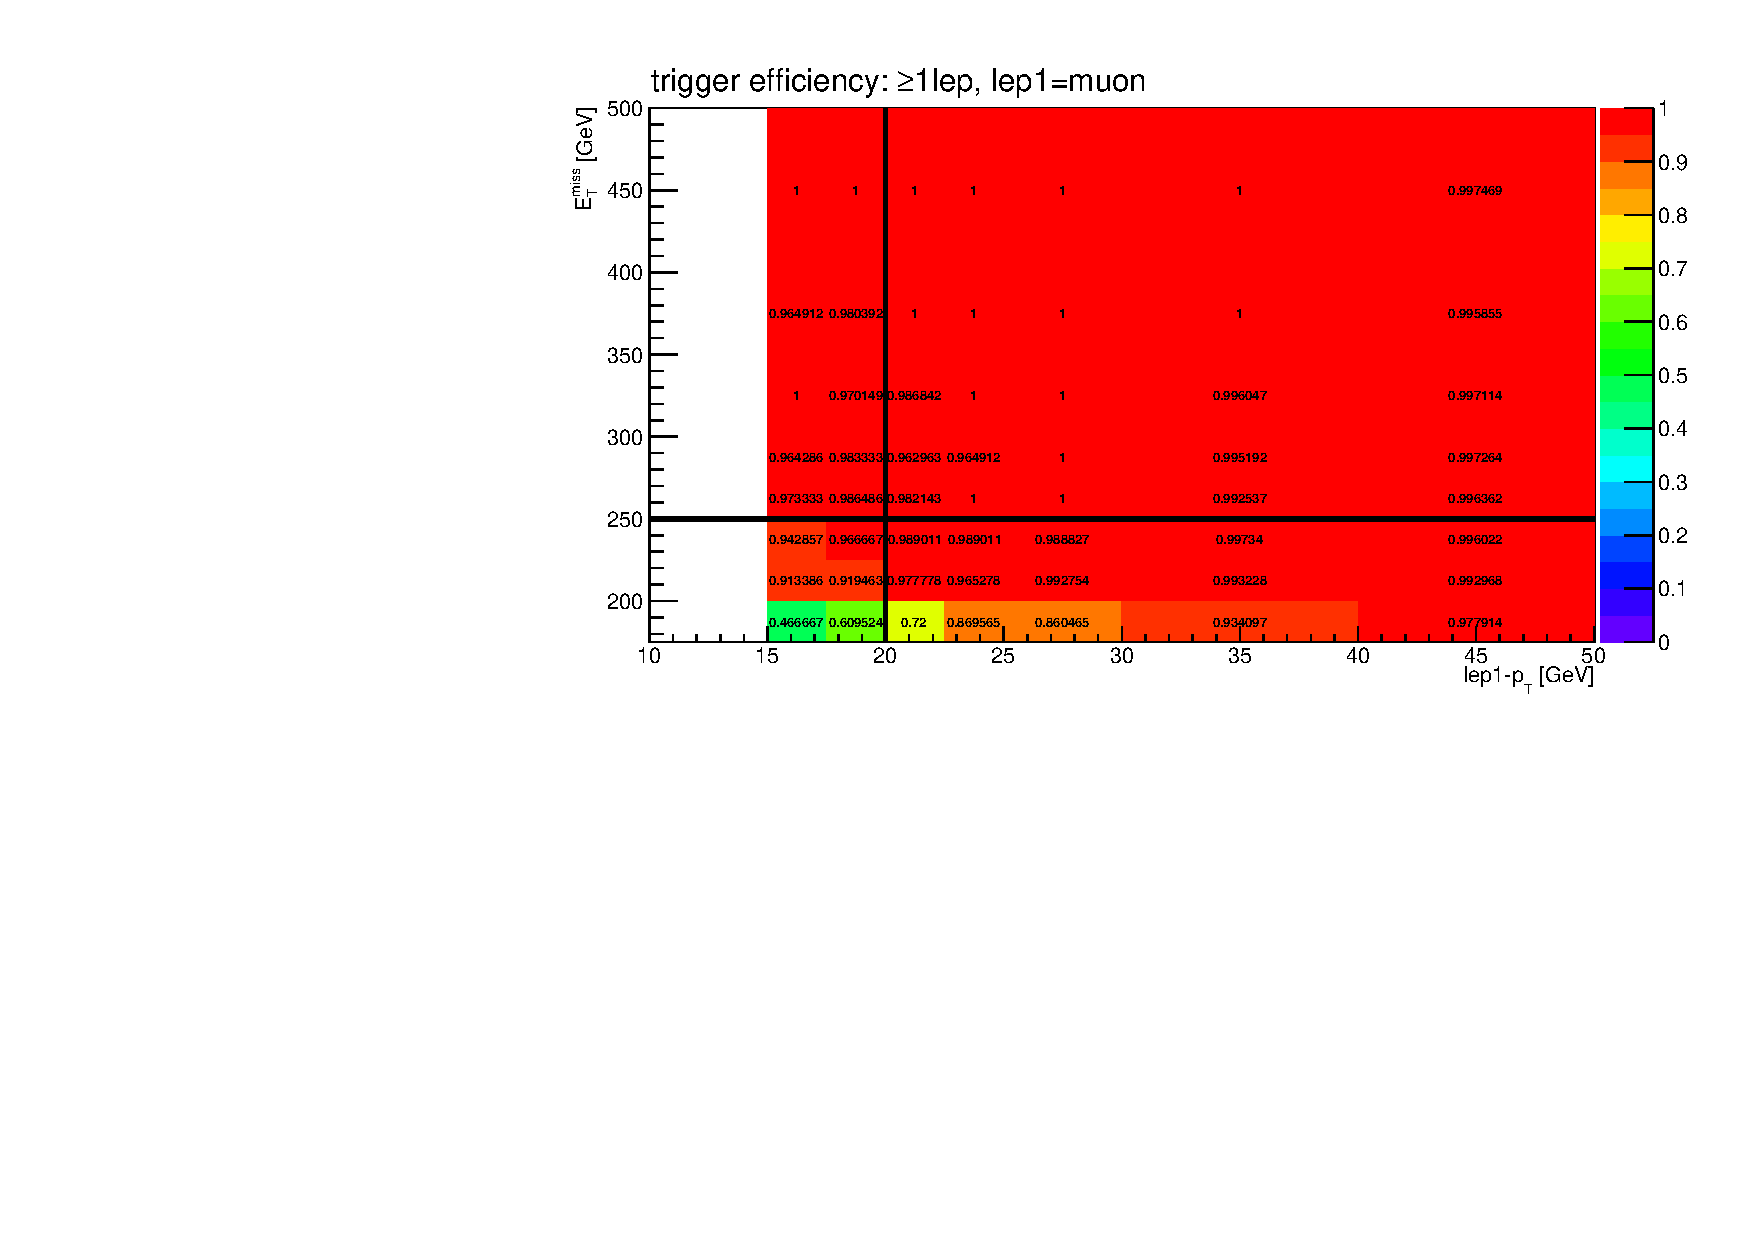
\includegraphics[width=0.45\textwidth]{figures/TriggerEff_mu.pdf}
\caption{Measured efficiencies for the union of the single lepton and
  $\met$ triggers. Efficiency is represented by the z-axis color scale. The
  efficiencies are presented separately for the case where the leading
  lepton is an electron (left), and a muon (right).}
\label{fig:stop:trigeff:1lepmet}
\end{figure}

As Section \ref{ssec:stop:lostlep} will describe, certain of our
background estimation techniques compel us to treat the $p_T$ of a
second lepton as part of the $\met$. For this special case, we must
re-evaluate the efficiency of our combined single lepton and $\met$
triggers. We do so using the exact same procedures described above,
except that we additionally require events to have a second lepton
with $p_T >$ 10 GeV. These efficiencies are presented in Figure
\ref{fig:stop:trigeff:2ndlepplusmet}. Because the combined triggers
have substantial inefficiency at low $\met$ and low lepton $p_T$, we
do correct our Monte Carlo simulations for these trigger
efficiencies when performing this background estimation.

% Plots of 2nd-lep-plus-met trigger efficiency taken from AN-16-463. Unpublished!
\begin{figure}[htb]
\centering
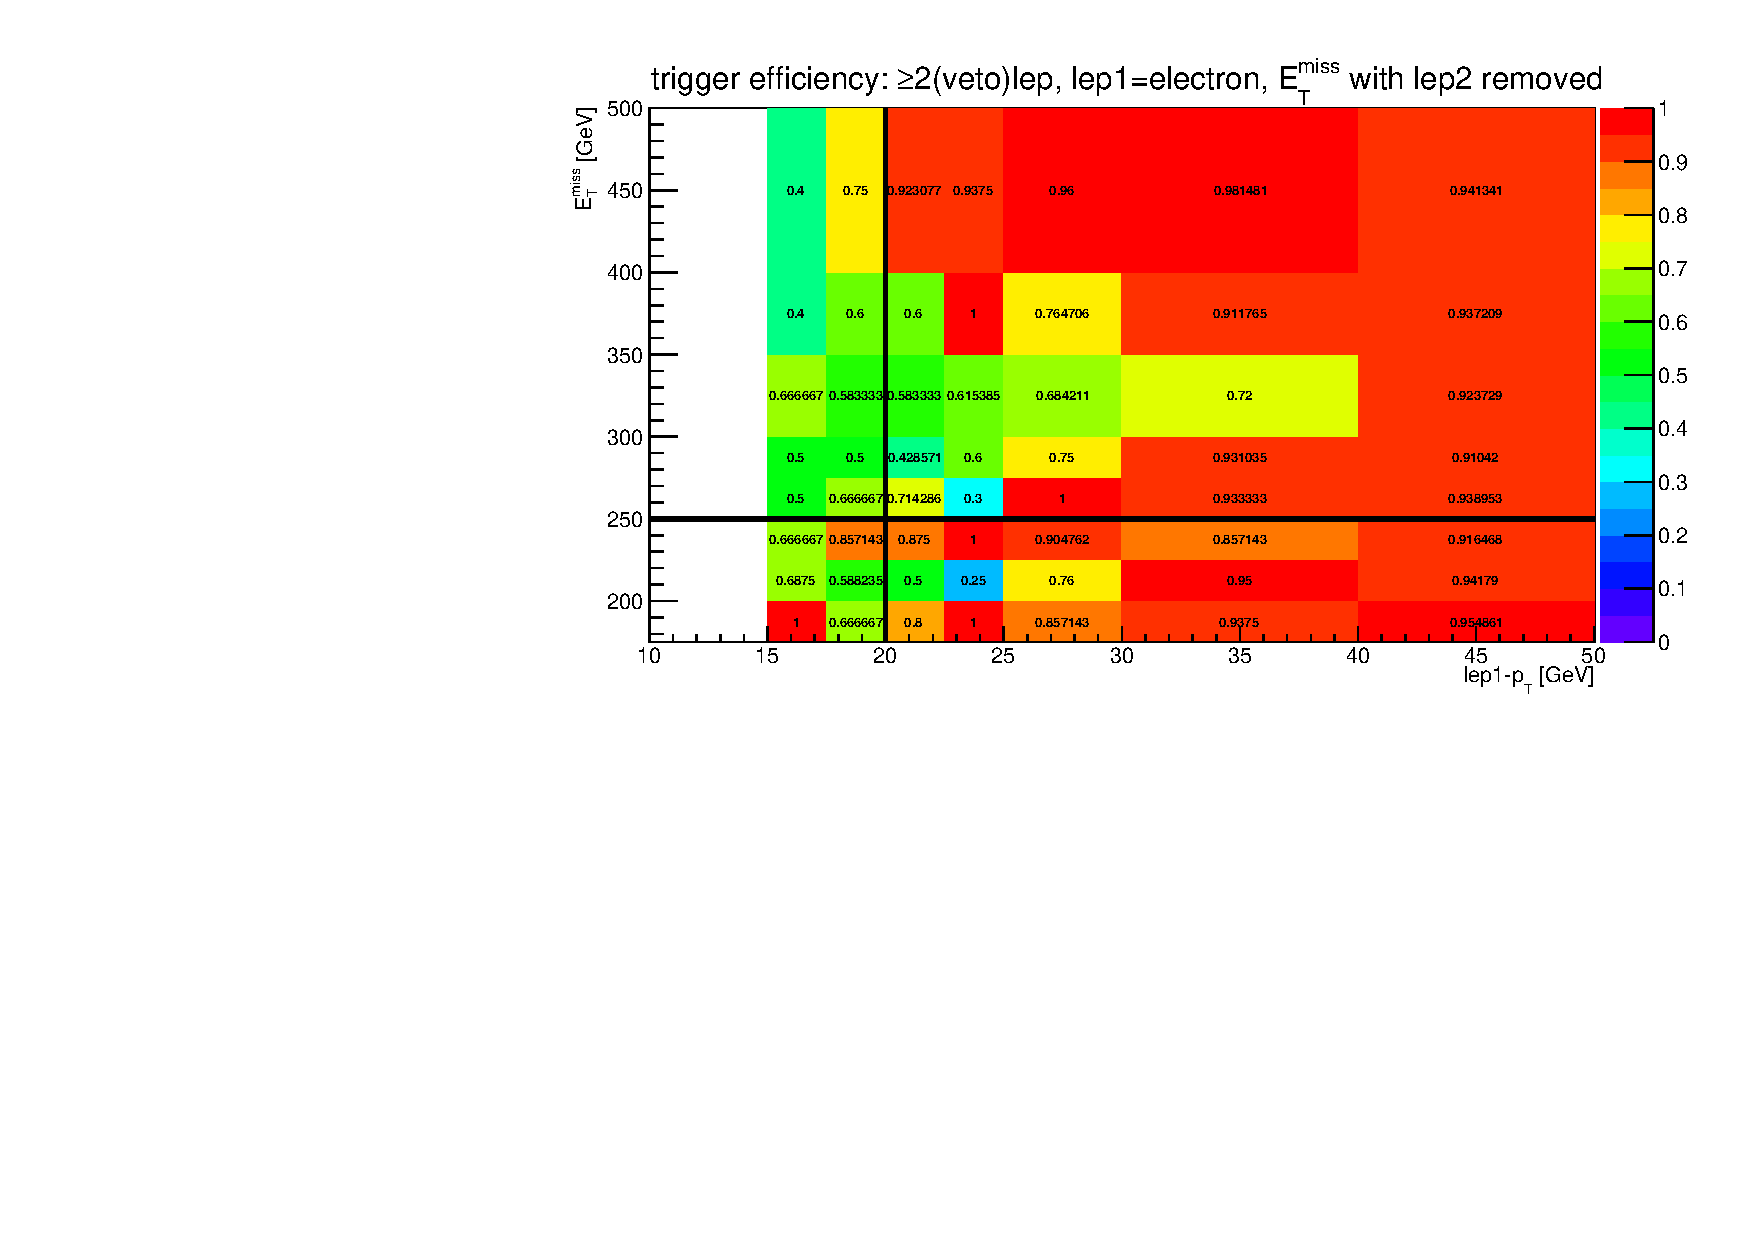
\includegraphics[width=0.45\textwidth]{figures/TriggerEff2l_el.pdf}
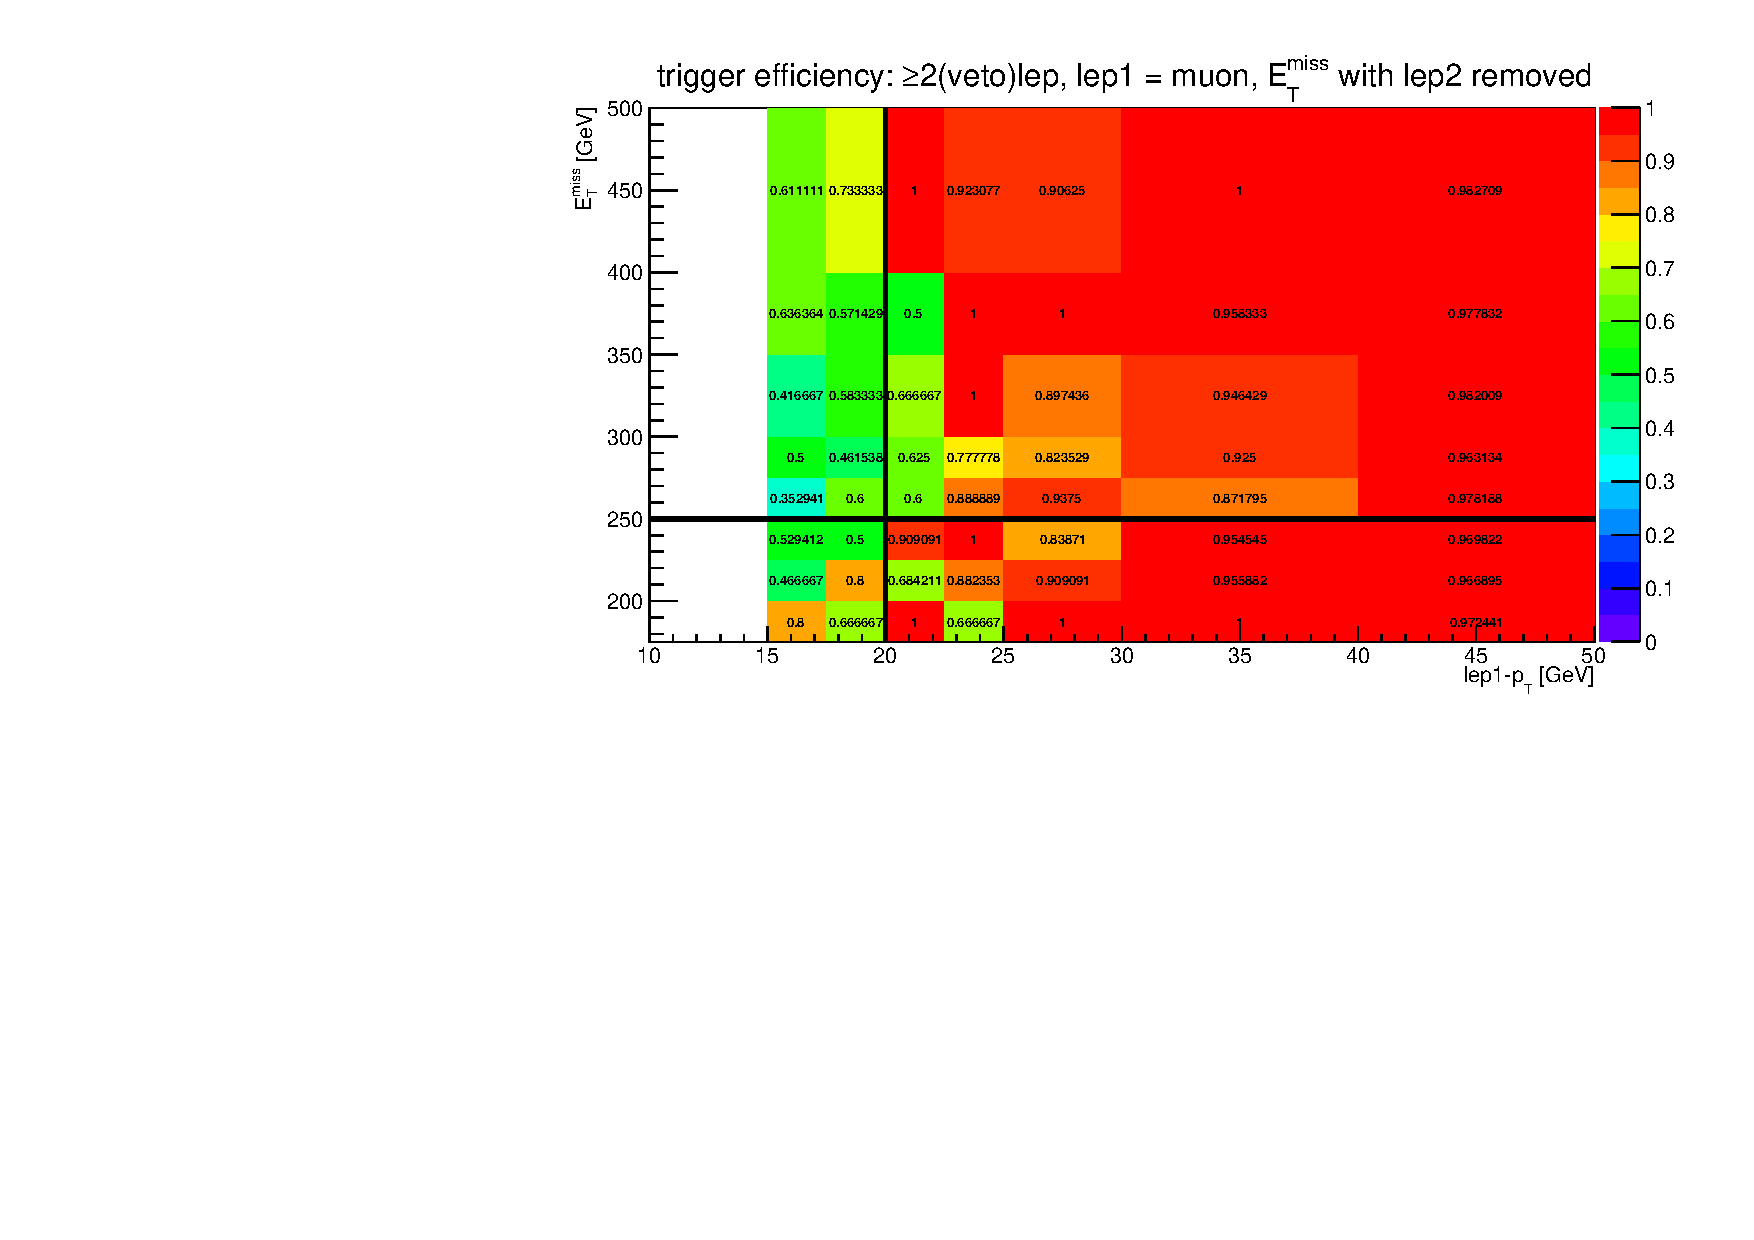
\includegraphics[width=0.45\textwidth]{figures/TriggerEff2l_mu.pdf}
\caption{Measured efficiencies for the union of the single lepton and
  $\met$ triggers, when the subleading lepton $p_T$ is added to the
  $\met$. Efficiency is represented by the z-axis color scale. The
  efficiencies are presented separately for the case where
  the leading lepton is an electron (left), and a muon (right).}
\label{fig:stop:trigeff:2ndlepplusmet}
\end{figure}

% What to say about the dilepton and single photon trigger
% efficiencies? How are these evaluated? Do we present measured
% efficiencies anywhere?

\subsection{Monte Carlo samples}
\label{ssec:stop:mcsamples}

Our analysis relies on modeling a number of background and signal
processes using Monte Carlo simulation. Table \ref{tab:stop:mcsamples}
presents the complete list of Monte Carlo samples used. All samples
are produced as MINIAODSIM.

% Table of MC samples taken from AN-16-463. Unpublished.
\begin{table}[htp]
\caption{
  Monte Carlo simulation datasets used in this analysis, and their
  theoretical cross sections. The symbol * replaces the string
  RunIISummer16MiniAODv2-PUMoriond17\_80X\_mcRun2\_asymptotic\_2016\_TrancheIV\_v6, % Warning: underfull hboxes abound here!
  and the $\dagger$ replaces
  RunIISpring16MiniAODv2-PUSpring16Fast\_80X\_mcRun2\_asymptotic\_2016\_miniAODv2\_v0.}
\label{tab:stop:mcsamples}
\centering
%\makebox[\textwidth][c]{%
{\footnotesize
\begin{tabular}{|l|c|c|c|}
\hline
Sample & Cross Section \\
& [pb] \\
\hline
/TTJets\_SingleLeptFromT\_TuneCUETP8M1\_13TeV-madgraphMLM-pythia8/*(\_ext)-v1 & 182.7 \\
/TTJets\_SingleLeptFromTbar\_TuneCUETP8M1\_13TeV-madgraphMLM-pythia8/*(\_ext)-v1 & 182.7 \\
/TTJets\_DiLept\_TuneCUETP8M1\_13TeV-madgraphMLM-pythia8/*\_ext-v1 (and *-v4) & 87.3 \\
/ST\_tW\_top\_5f\_NoFullyHadronicDecays\_13TeV-powheg\_TuneCUETP8M1/*-v1 & 19.6 \\
/ST\_tW\_antitop\_5f\_NoFullyHadronicDecays\_13TeV-powheg\_TuneCUETP8M1/*-v1 & 19.6 \\
/ST\_t-channel\_top\_4f\_leptonDecays\_13TeV-powheg-pythia8\_TuneCUETP8M1/*-v1 & 44.1 \\ 
/ST\_t-channel\_antitop\_4f\_leptonDecays\_13TeV-powheg-pythia8\_TuneCUETP8M1/*-v1 & 26.2 \\
/ST\_s-channel\_4f\_leptonDecays\_13TeV-amcatnlo-pythia8\_TuneCUETP8M1/*-v1 & 3.7 \\
/W1JetsToLNu\_TuneCUETP8M1\_13TeV-madgraphMLM-pythia8/*-v1 & 11782  \\
/W2JetsToLNu\_TuneCUETP8M1\_13TeV-madgraphMLM-pythia8/*-v1 & 3841 \\
/W3JetsToLNu\_TuneCUETP8M1\_13TeV-madgraphMLM-pythia8/*-v1 & 1160 \\
/W4JetsToLNu\_TuneCUETP8M1\_13TeV-madgraphMLM-pythia8/*-v1 & 600 \\
/W1JetsToLNu\_NuPt-200\_TuneCUETP8M1\_13TeV-madgraphMLM-pythia8/*-v1 & 2.36  \\
/W2JetsToLNu\_NuPt-200\_TuneCUETP8M1\_13TeV-madgraphMLM-pythia8/*-v1 & 4.95 \\
/W3JetsToLNu\_NuPt-200\_TuneCUETP8M1\_13TeV-madgraphMLM-pythia8/*-v1 & 4.94 \\
/W4JetsToLNu\_NuPt-200\_TuneCUETP8M1\_13TeV-madgraphMLM-pythia8/*-v1 & 8.83 \\
/ttWJets\_13TeV\_madgraphMLM/*-v1 & 0.61 \\
/ttZJets\_13TeV\_madgraphMLM/*-v1 & 0.78 \\
/WWTo2L2Nu\_13TeV-powheg/*-v1 & 12.18 \\
/WWToLNuQQ\_13TeV-powheg/*-v1 & 50.00  \\
/WZTo3LNu\_TuneCUETP8M1\_13TeV-powheg-pythia8/*-v1 & 4.43 \\
/WZTo2L2Q\_13TeV\_amcatnloFXFX\_madspin\_pythia8/*-v1 & 5.60 \\
/WZTo1L1Nu2Q\_13TeV\_amcatnloFXFX\_madspin\_pythia8/*-v1 & 10.74 \\
/WZTo1L3Nu\_13TeV\_amcatnloFXFX\_madspin\_pythia8/*-v1 & 3.05 \\
/ZZTo4L\_13TeV\_powheg\_pythia8/*-v1 & 1.25 \\
/ZZTo2L2Q\_13TeV\_amcatnloFXFX\_madspin\_pythia8/*-v1 & 3.22 \\
/ZZTo2L2Nu\_13TeV\_powheg\_pythia8/*-v1 & 0.56 \\
/ZZTo2Q2Nu\_13TeV\_amcatnloFXFX\_madspin\_pythia8/*-v1 & 4.73 \\
/SMS-T2tt\_mStop-150to250\_TuneCUETP8M1\_13TeV-madgraphMLM-pythia8/$\dagger$-v1 & \\
/SMS-T2tt\_mStop-250to350\_TuneCUETP8M1\_13TeV-madgraphMLM-pythia8/$\dagger$-v1 & \\
/SMS-T2tt\_mStop-350to400\_TuneCUETP8M1\_13TeV-madgraphMLM-pythia8/$\dagger$-v1 & \\
/SMS-T2tt\_mStop-400to1200\_TuneCUETP8M1\_13TeV-madgraphMLM-pythia8/$\dagger$-v1 & \\
/SMS-T2bW\_TuneCUETP8M1\_13TeV-madgraphMLM-pythia8/$\dagger$-v1 & \\
/SMS-T2bt\_TuneCUETP8M1\_13TeV-madgraphMLM-pythia8/$\dagger$-v1 & \\
\hline
\end{tabular}
}
\end{table}

% Transition between these sections by talking about the components
% other than 1L+MET used to identify stop decays?
\section{Search Strategy}
\label{sec:stop:searchstrategy}

Because we are searching for single lepton stop decays, we must select
events with one and only one lepton in them. In addition, the LSPs and
charginos should go undetected by the CMS detector; those sparticles
plus the neutrino should give relatively
large amounts of $\met$. Therefore, our main experimental signature is a
single lepton plus high $\met$.

Many other physics processes can produce a single lepton plus high
$\met$, or can produce signatures that resemble these. We must therefore
identify these backgrounds, and attempt to reduce their presence using
a series of cuts and selections. When it is not possible to mitigate
the backgrounds with cuts, we must attempt to estimate how many
background events fall into our signal regions so we can exclude them
from the final calculations.

In the absence of any particular cuts and selections, the largest
background will naturally be SM processes that produce one true lepton
and large $\met$. The notable example is $\ttonelep$,
though other processes contribute as well, such as W-boson production
with jets, where the W decays leptonically. In order to combat this
background component, we first add a cut on the transverse mass of the
lepton plus the $\met$, or $\mt$. The exact formula for this variable is
given by Equation \ref{eq:stop:mt} in Section \ref{ssec:stop:mt}. This cut works in
concert with our high-$\met$ requirement to help reduce the single-lepton
background component.

% Insert MT figures from AN

Figure \ref{fig:stop:mtstudies} shows the results of several
investigations into the $\mt$ variable. The left plot shows the
reconstructed value of $\mt$ in a sample of W($\ell\nu$)+jets MC
events, with three different $\met$ cuts applied. As the plot shows,
higher $\met$ requirements cause the W-boson mass edge to become more
sharply defined. % So? What does this really tell us?

The center plot shows generator-level $\mt$ and reconstructed $\mt$
for both W+jets and $\ttonelep$ simulated events. These
events were selected by requiring one single lepton and at least 2
jets, all with $p_T > 30$ GeV, and $\met >$ 250 GeV. The generator-level $\mt$ was
calculated using the neutrino momentum in place of the $\met$. The plot
shows that the tails of the $\mt$ distribution look very different for
W+jets and $\ttonelep$. In the case of $\ttonelep$, the top mass
restricts the mass spectrum of the W-boson, so that most events in the
tail are simply due to the limited resolution of $\met$
reconstruction. By contrast, in W+jets events, there is no constraint
on the W mass, so the tail is attributable to the natural width of the
W-boson mass spectrum. Thus, by selecting an appropriate $\mt$ cut, we
can effectively reduce the single lepton background to mostly W+jets
events. We can then estimate the size of the remaining background
component using techniques that will be described in Sections
\ref{ssec:stop:1lw} and \ref{ssec:stop:1ltop}. % Do I need to rewrite this to be clearer?

% Does the third plot actually show us anything? Is it important to
% include it?

After reducing the single lepton background using $\met$ and $\mt$ cuts,
the next largest background comes from events with two genuine
leptons, such as $\ttdilep$, where one of the leptons is not
reconstructed. As Section \ref{sec:stop:selections} will describe, we
veto events that have a second electron, muon, or tau, as well as
events with an isolated track in them. Nevertheless, these vetos are
not perfect. And often, a second lepton falls outside our range of
acceptance in $p_T$ or $\eta$, is not isolated, or is not
reconstructed. We call this component the ``lost lepton'' background,
and estimate it using techniques described in Section
\ref{ssec:stop:lostlep}.

The final background to consider is events with one genuine lepton,
but where the high $\met$ comes from a $Z \rightarrow \nu\nu$ decay,
and not from SUSY particles. The largest contributor to this
background is TTZ events, where the $\ttbar$ pair decays
semileptonically and the Z decays to invisible neutrinos; the next
largest contributor is WZ production. There is little we can do to
exclude such events with cuts; fortunately, this background component
is relatively small. We estimate the $Z \rightarrow \nu\nu$
component using MC with theoretical uncertainties applied, as
described in Section \ref{ssec:stop:rarebkg}.

\section{Object and Event Selection}
\label{sec:stop:selections}

% Give some intro paragraph here. Something that flows nicely.

\subsection{Vertex Selections}
\label{ssec:stop:vtxselections}

All events selected must have at least one good reconstructed
vertex. A vertex is considered to be ``good'' if it meets the
following criteria:

\begin{itemize}
\item The tracks used to create the vertex must have trajectory fits
  with positive $\chi^2$ values.
\item The vertex fit must have at least 5 degrees of freedom.
\item The distance between the vertex and the nominal center of the
  detector must have a $z$-component of less than 24 cm.
\item The same distance must have a transverse component, $\rho$, of
  less than 2 cm.
\end{itemize}

If multiple vertices in an event meet these criteria, we choose the
one whose associated tracks have the highest $\sum p_T^2$ to be our
primary vertex (PV), from which all of our physics objects originate.

\subsection{Lepton Selections and Veto}
\label{ssec:stop:lepselections}

We select events that have one well-identified reconstructed lepton
(electron or muon), and veto events with additional leptons. All our
identification criteria are based on the POG recommendations, and are
described in Table \ref{tab:stop:lepselections}.

For our electrons, we remove the POG-recommended isolation cut, and
substitute a cut based on \emph{relative mini-isolation}, as is standard for
SUSY searches at CMS. Relative mini-isolation is defined as the sum of
the $p_T$ of the particle flow candidates within a cone-shaped region
around the lepton, where the cone size varies with the lepton
$p_T$. For lepton $p_T <$ 50 GeV, the cone size is 0.2 in $\Delta
R$. For $p_T$ between 50 and 200 GeV, the cone size is defined to be
10.0 GeV / $p_T^{\text{lep}}$. Finally, for lepton $p_T$ above 200 GeV, the
cone size is fixed at 0.05. The rationale for reducing the cone size
as lepton $p_T$ rises is to avoid vetoing signal events
where a boosted top decays to a lepton and b-jet that are nearly
colinear. Pileup correction is performed using the average energy
density in the event, and the same effective area used in the
mini-isolation calculation.

\begin{table}[htb]
\centering
\caption{Criteria used to identify electrons or muons. We select
  exactly one good lepton, and veto any additional leptons, using two
  different sets of criteria.}
\label{tab:stop:lepselections}
\begin{tabular}{ l | l | c | c }
\hline
type & variable & selected & veto \\ \hline
\multirow{4}{*}{electron} &    $p_T$ & $>20$ GeV & $>5$ GeV \\
 &   $|\eta|$ & $<1.442$ & $<2.4$ \\
 &   POG ID without ISO & Medium & Veto \\
 &   relative miniisolation & $<0.1$ & $<0.2$ \\
 \hline
 \multirow{4}{*}{muon} &    $p_T$ & $>20$ GeV & $>5$ GeV \\
 &   $|\eta|$ & $<2.4$ & $<2.4$ \\
 &   POG ID & Medium & Loose \\
 &   relative miniisolation & $<0.1$ & $<0.2$ \\
\hline
\end{tabular}
\end{table}

\subsection{Isolated Track Veto}
\label{ssec:stop:isotrackveto}

In addition to vetoing events with a second electron/muon, we must
also reject events with a tau in them. Taus mostly decay in flight, so
to reject taus, we must reject their decay products. Some 50\% of the
time, taus decay to a charged pion or kaon. Decays to an electron and
a muon account for another 17.5\% each. Summing these cases up, we see
that 85\% of all tau decays produce a single charged track. So the
most powerful way to veto taus is to veto isolated charged
tracks. These tracks are found in the pfChargedHadrons collection. The
event is vetoed if at least one pfChargedHadron is found that meets these
criteria:
\begin{itemize}
\item $p_T >$ 10 GeV
\item $|\eta| <$ 2.4
\item Charge is opposite in sign from the selected lepton
\item $\Delta R >$ 0.4 from the selected lepton
\item $z$-component of the distance to the PV is $<$ 0.1 cm
\end{itemize}
We measure the isolation of a charged track using tracker-only
isolation, because tau decays sometimes produce multiple neutral
hadrons along with the charged track, and these hadrons should not be
counted against the track isolation. With that in mind, we require our
veto tracks to have the following isolation values:
\begin{itemize}
\item For track $p_T >$ 60 GeV, absolute tracker iso within a cone of
  0.3 must be $<$ 6 GeV.
\item For track $p_T \leq$ 60 GeV, relative tracker iso within a cone
  of 0.3 must be  $<$ 0.1.
\end{itemize}
Relative isolation is, again, isolation divided by the $p_T$ of the
object being considered. We use absolute isolation above $p_T$ of 60
GeV because relative isolation becomes a weak requirement at high
$p_T$.

\subsection{Hadronic Tau Veto}
\label{ssec:stop:hadtauveto}

Although highly effective, the isolated track veto does not address
cases where the tau decays to three charged hadrons (3-pronged
decay). So we add another veto targeting hadronic tau decays, using an
ID recipe approved by the tau POG within CMS. We veto events if we
find a hadronic tau that meets these criteria:

\begin{itemize}
\item $p_T >$ 20 GeV
\item $|\eta| <$ 2.4
\item Passes tau identification algorithm \emph{byDecayModeFinding}
\item Passes isolation selection
  \emph{byMediumCombinedIsolationDeltaBetaCorr3Hits}
\item Charge is opposite in sign from the selected lepton
\item $\Delta R >$ 0.4 from the selected lepton
\end{itemize}

\subsection{Jets}
\label{ssec:stop:jets}

We reconstruct jets using the anti-$k_t$ jet clustering algorithm
\cite{antikt} with a distance parameter of 0.4. These jets must have
$p_T >$ 30 GeV, must have $|\eta| <$ 2.4, and must pass the
established jet ID at the loose working point. The jet ID requirement
is waived for our signal MC samples, because the jet ID has some
inefficiencies in samples made using FastSim. We require a minimum of
two jets in every event; some signal regions have higher requirements to
suit their purposes, as Section \ref{sec:stop:sigregs} will describe.

We also require each event to have at least one b-tagged jet, where
b-tagging is performed using the CSVv2 algorithm. Depending on the
signal region in question, the b-tag may be required to pass the loose
WP (CSV $>$ 0.8) or the tight WP (CSV $>$ 0.935). Section
\ref{sec:stop:sigregs} will list which WP is used for each signal region.

\subsection{\texorpdfstring{$\met$}{MET}}
\label{ssec:stop:met}

As described earlier, $\met$ is calculated as the negative of the vector
sum of all the particle flow candidates in the event. We recalculate
the $\met$ after the jet energy corrections have been applied to the jets
in the event. We also employ the following filters, as recommended by
the JetMET group in CMS:

\begin{itemize}
\item Primary vertex filter
\item CSC beam halo filter
\item HBHE noise filter
\item HBHEiso noise filter
\item ee badSC noise filter
\item ECAL TP filter
\item Bad muon filter
\item Bad charged hadron filter
\item Bad muons filter
\item Duplicate muons filter
\end{itemize}

\subsection{Transverse Mass (\texorpdfstring{$\mt$}{MT})}
\label{ssec:stop:mt}

As alluded to in Section \ref{sec:stop:searchstrategy}, we use the
transverse mass of the lepton-$\met$ system to reduce the prevalence of
the single-lepton background, especially $\ttonelep$. By transverse
mass, we mean the solution to the relativistic equation $M^2 = E^2 -
p^2$, but using only the transverse components of the energy and
momentum of the lepton-$\met$ system. So:
\begin{equation}
\begin{split}
\mt^2 & = E_T^2 - p_T^2 \\
 & = (\met + E_\text{T}^\ell)^2 - (\vec{p}_\text{T}^\text{miss} + \vec{p}_\text{T}^\ell)^2
\end{split}
\end{equation}
Transverse energy is defined as:
\begin{equation}
E_\text{T}^2 = m^2 + p_\text{T}^2
\end{equation}
In the case of $\met$, the missing momentum and energy are the same
thing, giving us:
\begin{equation}
\mt^2 = m_\ell^2 + 2\met E_\text{T}^\ell - 2 \metvec \cdot \vec{p}_\text{T}^\ell
\end{equation}
In our case, $m_\ell$ is negligible compared to
$p_\text{T}^\ell$. This also means $E_\text{T}^\ell \approx p_\text{T}^\ell$.
So if $\phi$ denotes the transverse angle between $\metvec$ and
$\vec{p}_\text{T}^\ell$, then we find:
\begin{equation}
\label{eq:stop:mt}
\mt = \sqrt{2 \met p_\text{T}^\ell (1 - \cos \phi)}
\end{equation}

In events with an on-shell W-boson decaying to a single lepton and no
other sources of $\met$, the largest possible value $\mt$ can take on
is the W-boson mass, around 80 GeV. Thus, by cutting on $\mt$, we can
strongly reduce the presence of $ttonelep$, W+jets, and single-top
events. This fact is illustrated in Figure
\ref{fig:stop:mt:nminusone}. As described in Section
\ref{sec:stop:searchstrategy}, background events in the tail of the
$\mt$ distribution are mostly due to off-shell W-bosons and $\met$
resolution effects.

% MT n-1 plot, taken from AN-16-463. Believed unpublished.
\begin{figure}[htb]
\centering
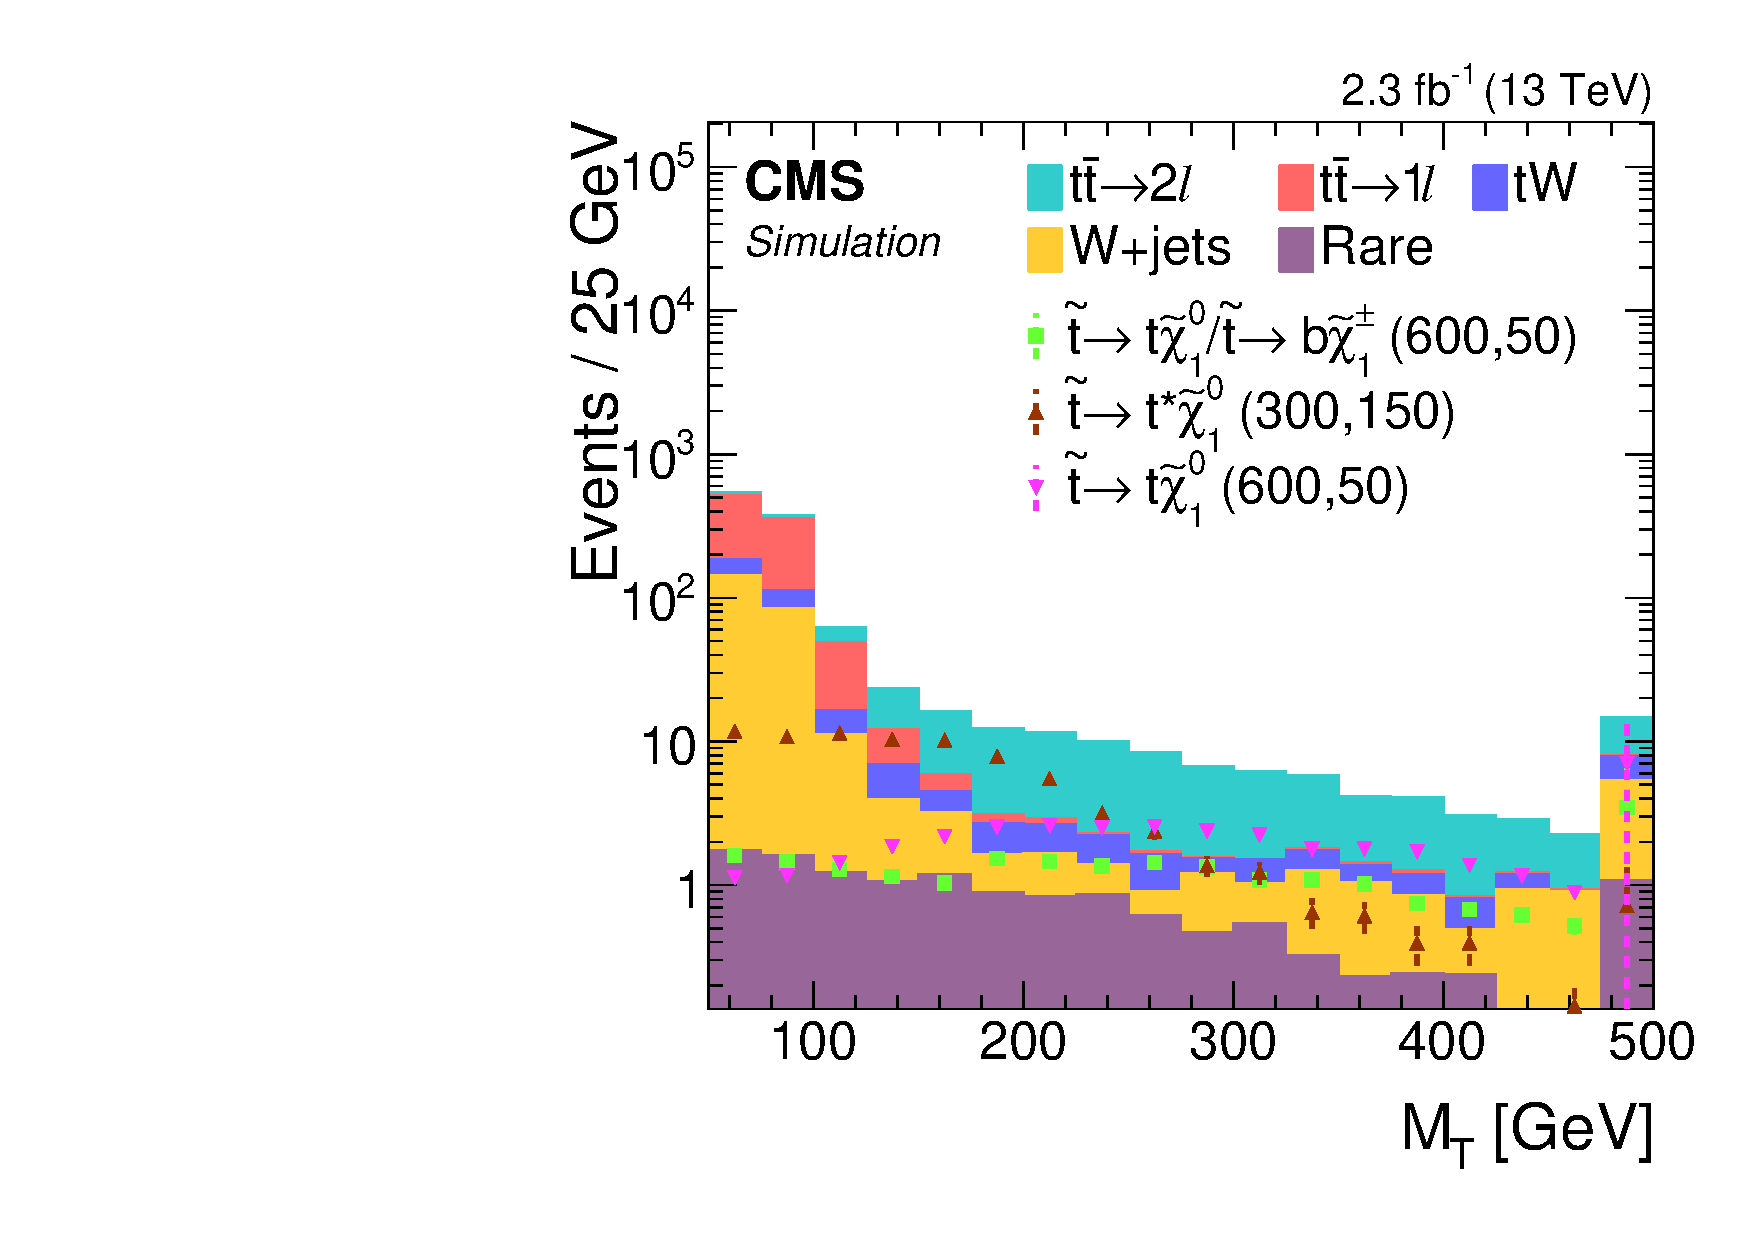
\includegraphics[width=0.5\textwidth]{figures/mt_nminusone.pdf}
\caption{Distribution of $\mt$ with all other event selections applied.}
\label{fig:stop:mt:nminusone}
\end{figure}

\subsection{Modified Topness (\texorpdfstring{$t_{\text{mod}}$}{tmod})}
\label{ssec:stop:tmod}

\subsection{Lepton-b Invariant Mass (\texorpdfstring{$m_{\ell b}$}{mlb})}
\label{ssec:stop:mlb}

\subsection{Minimum Delta-Phi (\texorpdfstring{$\text{min}\Delta\phi(j_{1,2},\met)$}{minDphi})}
\label{ssec:stop:mindphi}

% Corrections / SFs

Give the criteria we used to define electrons, muons, hadronic taus,
jets, b-tags, MET, etc.
% Also have to define M_T - a reference is expected above.
Talk about how we used these objects to select events.
Maybe this is a good place to also describe the scale factors and
other corrections applied to the Monte Carlo.

\section{Signal Regions}
\label{sec:stop:sigregs}

Give the definitions for the different signal regions.
Talk about why these definitions were chosen.

\subsection{Nominal Signal Regions}
\label{ssec:stop:nominalsrs}

\subsection{Corridor Signal Regions}
\label{ssec:stop:corridorsrs}



\section{Background Estimation}
\label{sec:stop:bkgest}

If you didn't do so earlier, go over the different backgrounds:
Lost lepton, 1l-from-W, 1l-from-top, and rare.

\subsection{Lost Lepton}
\label{ssec:stop:lostlep}

Introduce the dilepton control regions, and the selections used
to define them.
Talk about how these control regions are validated.
Describe how we do a data-driven estimate based on the CR yields.
Explain how we estimate all the various systematic uncertainties.

\subsection{Single Lepton not from Top}
\label{ssec:stop:1lw}

Talk about the single-lepton-from-W background.
Describe the WJets control regions and their selections.
Talk about validating these control regions.
Describe the data-driven estimate for this component.
Explain how the systematic uncertainties are calculated.

\subsection{Single Lepton from Top}
\label{ssec:stop:1ltop}

Explain how we take this background from Monte Carlo.
Describe the uncertainties we use to cover this estimate.

\subsection{Rare Standard Model Processes}
\label{ssec:stop:rarebkg}

Describe the rare background (particularly $TTZ \rightarrow \nu\nu$).
Talk about how this background is estimated.
Describe how systematics are assessed.

\section{Signal Estimate}
\label{sec:stop:signal}

Talk about how signal yields are estimated.
Describe the corrections for signal contamination in control regions.
Explain the method for assessing uncertainties on signal yields.

\section{Results}
\label{sec:stop:results}

Give the final yields and uncertainties.

\section{Limit Setting}
\label{sec:stop:limits}

Describe the Higgs Combine tool.
Talk about how we use it.
Explain (the rudiments of) the statistical methods.

\section{Interpretation}
\label{sec:stop:interp}

Maybe combine with previous section?
Anyway, interpret our results in the context of constraints on stop production.

